\documentclass[11pt,a4paper]{article}

\usepackage[T1]{fontenc}
\usepackage[utf8]{inputenc}
\usepackage{lmodern}
\usepackage[margin=2.5cm]{geometry}
\usepackage{amsmath}
\usepackage{booktabs}
\usepackage{threeparttable}
\usepackage{graphicx}
\usepackage{caption}
\usepackage[authoryear,round]{natbib}
\usepackage{setspace}
\usepackage[hidelinks]{hyperref}

\captionsetup{font=small,labelfont=bf}
\setstretch{1.15}
\newcommand{\Kstar}{K^{*}}

\title{\textbf{Option Expirations and the Closing Price}\\[4pt]
\large Delta hedging, pinning and closing-auction prices in US equities, 2016--2025}
\author{Luca Dennert\\[2pt]
\small MSc in Finance, Universit\`a Bocconi\\
\small Essay for 21048 Market Structure and Information-Based Models (Prof.\ Barbara Rindi)}
\date{November 2026}

\begin{document}
\maketitle

\begin{abstract}
\noindent US equity options settle on the closing-auction price, so dealers' delta hedging on expiration days flows into the most important price of the day. Using 7.6 million stock-days from 2016 to 2025 and expiring open interest from OptionMetrics, I compare stocks on the same day with more and less expiring gamma or open interest relative to their normal volume. Closes cluster at the strike with the largest expiring open interest. Controlling for how far each stock starts from that strike, the probability of closing within 0.25\% of it rises with expiring open interest relative to volume, and this gradient is 3.6--3.8 percentage points steeper ($t>6$) than for a placebo strike that does not expire, whose own gradient is negative. Among optionable stocks, high expiring gamma also makes the closing move about 0.4--0.9~bp smaller, while having options expire has no effect on its own once size and liquidity are controlled for. Closing moves reverse overnight by 43--58\% on all types of day, with no extra reversal on expiration days. The pattern is consistent with hedging by dealers who are net long gamma. A test of the 2022 daily SPX expirations is not informative.
\end{abstract}

\section{Introduction}

Does the hedging of expiring options distort the most important price of the trading day? The closing auction sets the price used for fund valuations, index levels and benchmarks, and it is also the price on which US equity options settle. On an expiration day, dealers who sold or bought those options must rebalance their stock hedges, and much of that rebalancing reaches the close. If the flow is large relative to the liquidity in the auction, the closing price could move away from fundamental value precisely when the most money depends on it.

This essay takes the question to 7.6 million stock-days of US common stocks between 2016 and 2025, combining CRSP prices with expiring open interest from OptionMetrics. The design follows the closing-auction analysis of \citet{ComertonFordeRindi2022}, which asks whether large closing-price changes are price discovery or temporary dislocation, and the pinning evidence of \citet{NiPearsonPoteshman2005}. The new element is a measure of hedging pressure, \emph{gamma intensity}: the dollar gamma of the options that expire on a given day relative to the stock's normal dollar volume. Comparing stocks with high and low gamma intensity on the same day removes everything that affects all stocks on expiration Fridays.

Three findings stand out. First, closing prices cluster at the strike with the largest expiring open interest. Gamma is mechanically high when the price starts near a strike, so the main tests compare stocks that start equally far from their strike and measure hedging pressure with open interest alone. On this basis the probability of closing within 0.25\% of the strike rises by 2.2 percentage points from the lowest- to the highest-OI expirations of a day, whereas it falls by 1.4~pp across the same range on Fridays when the strike does not expire: a difference in gradients of 3.6~pp ($t=6.1$). With gamma instead of open interest, and the same distance controls, the gradient among expirations is 3.3~pp. Second, among stocks with listed options, high expiring gamma makes the closing move smaller by about 0.4--0.9~bp, a tenth to a sixth of its size. Having options expire does not change the closing move on its own; an apparently larger effect in the full sample comes from comparing optionable stocks with small, illiquid ones. Third, closing moves measured by the proxy reverse overnight by 43--58\% on every type of day, but not more on expiration days or after high-gamma expirations. A triple difference on the 2022 SPX Tuesday and Thursday expirations is matched by its placebo and is therefore uninformative.

Together the results are consistent with dealers who are net long gamma and whose hedging pins prices near large strikes without destabilising the close. They do not show that the hedging-related part of the close is permanent, and they rely only on daily data; Section~\ref{sec:limits} discusses what intraday data would add.

\subsection*{Related literature}

The results are consistent with the existing evidence and extend it to the period of weekly and daily options.

\paragraph{Stock pinning.} \citet{AvellanedaLipkin2003} show in a model that delta hedging of large long-option positions can pin the price at the strike. \citet{NiPearsonPoteshman2005} document that optionable US stocks cluster at strike prices on expiration Fridays in 1996--2002, and attribute it to market makers' re-hedging and to manipulation by proprietary traders. This essay finds the same attraction in 2016--2025 and ties its strength to a continuous measure of expiring gamma.

\paragraph{The sign of dealer positions.} \citet{GolezJackwerth2012} find that S\&P~500 futures are pulled towards the at-the-money strike when options on the futures expire, but pushed away from it before S\&P~500 index options expire, where market makers are net short. The direction of the effect depends on dealers' net gamma, the same logic used here to read the single-stock results as long-gamma hedging.

\paragraph{Daily expirations and volatility.} \citet{Adams0DTE} find that zero-day (0DTE) S\&P~500 options dampen index volatility on average, through market makers' hedging needs, and use the Tuesday and Thursday expirations before May 2022 as a source of variation. Smaller closing moves on high-gamma expiration days are consistent with that mechanism at the stock level; the essay's own SPX test (Section~\ref{sec:spx}) is not informative enough to add to it.

\paragraph{Settlement on the open.} \citet{BaltussenTersteggeWhelan2024} show that the special opening quotation used to settle AM-settled S\&P~500 derivatives on third Fridays exceeds the previous close by about 18~bp on average and reverts by about midday. The earlier version of their paper argued that the pattern is hard to explain without manipulation of the settlement price. Either way, settlement on the open is not free of expiration-related price pressure.

\paragraph{Closing auctions.} \citet{ComertonFordeRindi2022} study European closing auctions and find that auction returns, measured from the last continuous trade, are permanent in liquid stocks and only slightly reversed the next day in less liquid ones, so that auctions are important price-discovery events. \citet{BogousslavskyMuravyev2023} and \citet{HuMurphy2026} study who trades at the close and how it affects closing prices in the US. This essay applies the same discovery-versus-dislocation logic to the specific flow that expiring options bring to the auction.

The contribution is therefore not a new phenomenon but a sharper test of an old one: a same-day comparison across stocks, with controls for how close each stock starts to the strike and a placebo strike whose open-interest gradient can be estimated in the same way.

\section{Institutional background}

\paragraph{The closing auction sets the most-used price of the day.} On NYSE and Nasdaq, continuous trading ends at 16:00 ET with a call auction (the NYSE closing auction and the Nasdaq Closing Cross). The resulting official closing price is the benchmark for fund NAVs, index levels and performance measurement, and closing auctions now account for more than 10\% of US equity volume \citep{HuMurphy2026}.

\paragraph{Equity options settle on that price.} Single-stock options are American-style and physically settled. At expiration, exercise is decided by whether the option is in the money at the close, so the closing price of the expiration day determines which contracts become stock positions. Standard monthly contracts expire on the third Friday; weekly contracts on many underlyings expire on the other Fridays. When the Friday is a market holiday, expiration moves to Thursday.

\paragraph{Index options use two settlement conventions.} Monthly S\&P~500 (SPX) options are AM-settled, on a special opening quotation of the third Friday. SPX Weeklys (SPXW) are PM-settled at the close. Before 2022, SPXW expired on Mondays, Wednesdays and Fridays. Cboe added Tuesday expirations from 18 April 2022 and Thursday expirations from 11 May 2022, so that an SPX contract now expires at the close of every trading day \citep{Cboe2022}.

\paragraph{Option dealers hedge their delta in the underlying.} A market maker who is long gamma must sell the stock when it rises and buy when it falls; a short-gamma dealer does the opposite. Gamma is largest for near-the-money contracts close to expiration, so on an expiration day the hedging flow for strikes near the current price can be large relative to normal volume. Much of this rebalancing can be executed at the close, through market-on-close orders that interact with the auction.

\section{Theory and hypotheses}

\paragraph{Hedging flow is uninformed but predictable order flow, and a call auction prices it.} In a batch-clearing market in the spirit of \citet{Kyle1985}, the clearing price moves with net order flow because liquidity suppliers cannot tell informed from uninformed demand. Delta-hedging orders carry no information about fundamentals, yet they arrive in the closing auction in size and in a predictable direction. Absent enough competing liquidity, they move the closing price away from its efficient value, and the move should reverse once the pressure is gone. This is the discovery-versus-dislocation distinction that \citet{ComertonFordeRindi2022} apply to closing auctions.

\paragraph{The sign of the dealer's gamma decides the direction of the pressure.} Models of stock pinning \citep{AvellanedaLipkin2003} show that delta hedging by long-gamma market makers pushes the price towards strikes with large open interest: they sell above the strike and buy below it. Short-gamma dealers trade with the move and push the price away from the strike. \citet{NiPearsonPoteshman2005} find that optionable US stocks cluster at strike prices on expiration Fridays, and attribute the effect mainly to the hedging of market makers who are net long options. \citet{GarleanuPedersenPoteshman2009} show that end users are on average net short single-stock options, which leaves dealers net long. The baseline prediction for single stocks is therefore attraction towards strikes.

\paragraph{Testable predictions.}
\begin{enumerate}
\item[\textbf{H1}] \textbf{(Attraction.)} On a stock's expiration day, the closing price moves towards the strike with the largest expiring open interest, and more so when expiring gamma is large relative to the stock's normal dollar volume.
\item[\textbf{H2}] \textbf{(Placebo.)} On Fridays when the stock has no options expiring, there is no comparable attraction towards the max-OI strike of the next expiration, and no positive gradient in its open interest.
\item[\textbf{H3}] \textbf{(Dislocation.)} The part of the closing move driven by hedging reverses overnight: the next-day open undoes part of it, more so on expiration days with high gamma.
\item[\textbf{H4}] \textbf{(Index expirations.)} When SPX options began to expire at the close on Tuesdays and Thursdays in 2022, closing-price dislocation of S\&P~500 members rose on those days relative to comparable non-members and to other weekdays.
\end{enumerate}

\section{Data and variable construction}

\paragraph{Sample.} The sample covers 7.59 million stock-days of 6,245 US common stocks from January 2016 to 29 August 2025. The end date is the last day of OptionMetrics on WRDS. Stock data come from the CRSP v2 daily file: ordinary common shares of US-incorporated firms listed on NYSE, Nasdaq or NYSE American, with a previous close above \$5. Option data come from OptionMetrics IvyDB US and are matched to CRSP through the WRDS link table, keeping only matches with score~1, the best of the table's six quality levels, within each link's validity dates. The 19 NYSE early-close days (13:00 closes around Independence Day, Thanksgiving and Christmas) are dropped from all expiration-day tests, because the auction takes place at a different time. The sample contains 504 expiration dates and 422,889 stock-expiration observations, of which 283,526 are standard (monthly) and 139,363 weekly expirations.

\paragraph{Expiring open interest.} For every stock and expiration date I take all contracts that expire that day. OptionMetrics reports open interest with a one-day lag, so the figure on the expiration date is the open interest at the previous close, the position dealers carry into the expiration day. The \emph{max-OI strike} $\Kstar$ is the strike with the largest combined call and put open interest.

\paragraph{Gamma intensity.} OptionMetrics leaves gamma missing on the expiration day and often on the day before, so I recompute Black--Scholes gamma with one trading day to expiry ($T=1/252$). All inputs are taken at the previous close, so they are known before the expiration day: the underlying price $S_{t-1}$, the contract's implied volatility on day $t-1$ (or, when it is missing, the median implied volatility of that day's expiring strikes within $\pm10\%$ of the price), and open interest. Contracts are treated as standard 100-share contracts; adjusted contracts created by corporate actions, whose deliverable differs, are not removed. They sit at non-standard strikes and usually carry little open interest, so they add noise to gamma intensity rather than bias; removing them would require the special-settlement flag, which the extraction did not keep. Expiring dollar gamma is
\begin{equation}
\mathrm{DG}_{i,t} = \sum_{j} \Gamma_{j}\times \mathrm{OI}_{j}\times 100\times S_{i,t-1}^{2}\times 0.01,
\end{equation}
the dollar value of shares a hedger trades for a 1\% move. Gamma intensity divides it by the stock's average daily dollar volume over the previous 20 days. Its median is 0.9\% of daily volume and its 90th percentile 4.9\%. Regressions use its percentile rank within each expiration date, from 0 to 1, so that the coefficient compares the highest- to the lowest-gamma expirations of the same day.

\paragraph{Outcomes.} The \emph{closing-price move} is the auction-return proxy $\log(P^{\text{close}}/M)$, where $M$ is the midpoint of CRSP's closing bid and ask (Section~\ref{sec:limits} and Appendix~\ref{app:proxy} discuss its validity). The \emph{overnight return} is $\log(P^{\text{open}}_{t+1}/P^{\text{close}}_{t})$, the reversal measure of \citet{ComertonFordeRindi2022}. \emph{Pinning} is measured by whether the close lies within 0.10\% or 0.25\% of $\Kstar$. Returns are expressed in basis points and winsorised at the 1st and 99th percentiles. The CRSP closing price is the auction price itself: \citet{BogousslavskyMuravyev2023} find that it equals the closing-auction price in 99.99\% of observations from 2014.

\paragraph{Data that are not available.} WRDS at Bocconi does not include TAQ, and LSEG Tick History is not available for this project. The essay therefore observes the official closing price and the next open exactly, but not the intraday quotes just before the auction, the auction volume or the order imbalance. It also does not observe who holds the options, so the sign of dealer positions is inferred rather than measured.

\section{Empirical design}
\label{sec:design}

\paragraph{Identification.} Third Fridays coincide with futures expiration, index rebalancing and other events that move all closing prices together. Identification therefore comes from differences across stocks on the same day, not from comparing expiration days with other days. Every regression includes date fixed effects, which absorb anything common to a given day, and stock fixed effects, which absorb a stock's average liquidity. Standard errors are clustered by stock and by date.

\paragraph{Baseline specification.} The estimating sample is the set of Fridays, plus Thursdays when an expiration falls on them. On each such day a stock either has options expiring (treated) or not: it may have no listed options, or only monthly options in a week without a monthly expiration. The baseline specification is
\begin{equation}
y_{i,t} = \beta_1\,\mathrm{Exp}_{i,t} + \beta_2\,\mathrm{Exp}_{i,t}\times \mathrm{GammaRank}_{i,t} + \gamma' X_{i,t} + \alpha_i + \delta_t + \varepsilon_{i,t},
\end{equation}
where $\mathrm{Exp}_{i,t}$ is one when stock $i$ has options expiring on day $t$, $\mathrm{GammaRank}_{i,t}$ is the percentile rank of gamma intensity among that day's expiring stocks, and $X_{i,t}$ holds log market capitalisation, log dollar volume, the closing half-spread and 20-day return volatility. The coefficient $\beta_2$ measures how much the outcome differs between the highest- and lowest-gamma expirations of the same day.

\paragraph{Placebo strike.} For treated stock-days $\Kstar$ is the max-OI strike of the expiring contracts. For untreated Fridays of optionable stocks it is the max-OI strike of the \emph{next} expiration, a strike of the same kind that carries no expiring hedge. The pinning sample is restricted to stock-days whose previous close lies within 2\% of $\Kstar$ (1\% in a robustness check).

\paragraph{Pinning without the mechanical link between gamma and distance.} Gamma is largest when the price starts near the strike, and a stock that starts near the strike is more likely to close near it for purely mechanical reasons. A gamma-based gradient can therefore pick up starting distance rather than hedging. The main pinning specification removes this channel in two ways. First, it adds fixed effects for 10-bp bins of the starting distance $|P_{t-1}-\Kstar|/\Kstar$, interacted with terciles of 20-day volatility, so that stocks are compared only with stocks that start equally far from their strike and move equally much. Second, it replaces gamma with \emph{OI intensity}: open interest at $\Kstar$ in shares divided by the stock's average daily share volume over the previous 20 days. Unlike gamma, OI intensity does not depend on the starting distance, and it can be computed in the same way for the placebo strike (with the next expiration's open interest). Its percentile rank is taken across all stock-days of the same date, treated and placebo together, and the specification is
\begin{equation}
\mathrm{Pin}_{i,t} = \beta_1\,\mathrm{Exp}_{i,t} + \beta_2\,\mathrm{OIRank}_{i,t} + \beta_3\,\mathrm{Exp}_{i,t}\times\mathrm{OIRank}_{i,t} + \mu_{d(i,t),v(i,t)} + \alpha_i + \delta_t + \varepsilon_{i,t},
\end{equation}
where $\mu_{d,v}$ are the distance-by-volatility fixed effects. $\beta_2$ is the open-interest gradient on Fridays without expiring options, where no hedge is unwound, and $\beta_3$ is how much steeper the gradient is when the options do expire. H1 predicts $\beta_3>0$; H2 predicts $\beta_2\le 0$.

\paragraph{SPX triple difference.} For 2021 to mid-2023, Monday to Thursday, the test compares S\&P~500 members with optionable non-members above \$2 billion of market capitalisation, Tuesdays and Thursdays with Mondays and Wednesdays (which already had SPX expirations), before and after the 2022 introduction. A placebo moves the introduction date back by one year.

\section{Results}

\subsection{Descriptive statistics}

Stocks with expiring options are larger and more liquid than the rest of the sample (Table~\ref{tab:desc}), which is why all tests rely on stock and date fixed effects.

\begin{table}[ht]
\centering
\begin{threeparttable}
\caption{Descriptive statistics, Fridays and expiration Thursdays}
\label{tab:desc}
\footnotesize
\setlength{\tabcolsep}{4pt}
\begin{tabular}{lrrrrrr}
\toprule
 & Stock-days & Stocks & $|$Closing move$|$ & $|$Overnight$|$ & Half-spread & Mkt cap \\
 & & & (bp) & (bp) & (bp, median) & (\$bn, median) \\
\midrule
Options expiring that day & 422,889 & 4,680 & 6.3 & 81.8 & 2.4 & 4.49 \\
Optionable, none expiring & 840,216 & 4,526 & 8.0 & 77.0 & 3.9 & 1.74 \\
No listed options & 310,334 & 3,267 & 40.8 & 100.0 & 37.4 & 0.18 \\
\bottomrule
\end{tabular}
\begin{tablenotes}\footnotesize
\item Sample: CRSP common stocks, January 2016 -- 29 August 2025, previous close above \$5. Means unless stated.
\end{tablenotes}
\end{threeparttable}
\end{table}

\subsection{Pinning (H1 and H2)}

Figure~\ref{fig:pin} shows the raw pattern. In the top quintile of gamma intensity, 12.8\% of closes land within 0.25\% of $\Kstar$, against 9.6\% in the bottom quintile and 9.7\% for the placebo strike. Table~\ref{tab:pin} gives the first-pass regressions. The coefficient of 4.5 percentage points on Expiring~$\times$~GammaRank is a \emph{gradient}: it compares the highest- with the lowest-gamma expirations of the same day. Because the lowest-gamma expirations sit slightly below the placebo ($-0.9$~pp), the top-gamma expirations exceed the placebo by about 3.6~pp ($-0.9+4.5$), or roughly a third of the placebo rate.

\begin{figure}[ht]
\centering
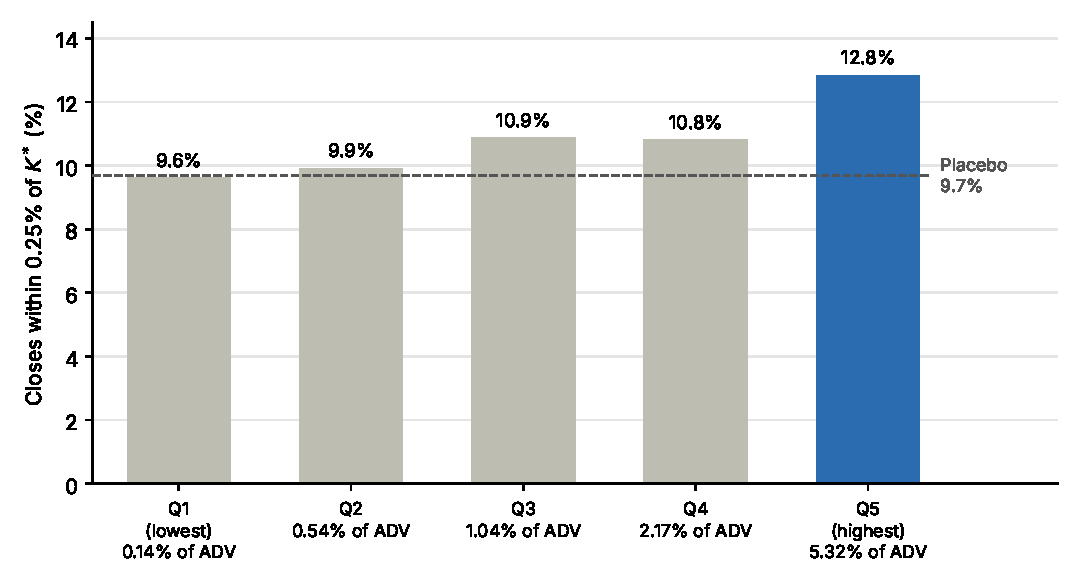
\includegraphics[width=0.92\textwidth]{figures/pinning_by_gamma.pdf}
\caption{Share of expiration-day closes within 0.25\% of the max-OI strike, by quintile of gamma intensity. Stocks whose previous close was within 2\% of $\Kstar$. The dashed line is the placebo rate: Fridays without expiring options, using the next expiration's max-OI strike (117,737 stock-days). Labels under the bars give the median expiring dollar gamma as a percentage of 20-day average dollar volume.}
\label{fig:pin}
\end{figure}

\begin{table}[ht]
\centering
\begin{threeparttable}
\caption{Pinning at the max-OI strike (percentage points)}
\label{tab:pin}
\small
\begin{tabular}{lcccc}
\toprule
 & \multicolumn{2}{c}{Previous close within 1\%} & \multicolumn{2}{c}{Previous close within 2\%} \\
\cmidrule(lr){2-3}\cmidrule(lr){4-5}
Close within & 0.10\% & 0.25\% & 0.10\% & 0.25\% \\
\midrule
Options expiring & $-1.2$ & $-0.9$ & $-1.0$ & $-0.9$ \\
 & $(-2.6)$ & $(-1.5)$ & $(-3.3)$ & $(-2.5)$ \\
Expiring $\times$ GammaRank & \textbf{2.0} & \textbf{3.4} & \textbf{2.8} & \textbf{4.5} \\
 & $(3.3)$ & $(4.2)$ & $(7.0)$ & $(8.3)$ \\
\midrule
Placebo rate & 5.6\% & 12.7\% & 4.3\% & 9.7\% \\
Stock-days & 105,894 & 105,894 & 204,619 & 204,619 \\
\bottomrule
\end{tabular}
\begin{tablenotes}\footnotesize
\item Linear probability models with stock and date fixed effects; controls: closing half-spread and 20-day volatility. $t$-statistics in parentheses, standard errors clustered by stock and date. First-pass specification; Table~\ref{tab:pinrob} removes the mechanical link between gamma and starting distance.
\end{tablenotes}
\end{threeparttable}
\end{table}

In this first pass the effect holds for standard monthly expirations (6.0 pp, $t=8.6$) and, more weakly, for weekly ones (2.4 pp, $t=2.9$), and it is similar in 2016--2019 (5.1 pp, $t=5.9$) and 2020--2025 (4.3 pp, $t=6.1$).

\paragraph{The attraction survives controls for starting distance, and the placebo has no positive gradient.} Table~\ref{tab:pinrob} reports the specifications of Section~\ref{sec:design} that remove the mechanical link between gamma and starting distance (early-close days excluded). Adding distance-by-volatility fixed effects lowers the gamma gradient from 4.5 to 3.3~pp ($t=6.2$): about a quarter of the first-pass estimate reflected how close high-gamma stocks start to the strike. With OI intensity, which does not depend on the starting distance, the placebo gradient is \emph{negative} ($-1.4$~pp, $t=-3.8$): on Fridays without expiring options, stocks with more open interest at the next expiration's top strike are, if anything, less likely to close near it. On expiration days the gradient is 3.6~pp steeper ($t=6.1$), and 3.8~pp ($t=6.4$) when date fixed effects are interacted with size deciles. The same holds for the 0.10\% band. It also holds for stocks that start between 0.25\% and 1\% from $\Kstar$, which are outside the target band at the previous close and must move into it during the day (3.4~pp, $t=3.3$, column~5). On these estimates the top-gamma, or top-OI, expirations close within 0.25\% of $\Kstar$ about 2.5~pp more often than placebo stock-days with the same OI rank and starting distance ($-1.0+3.6$), a quarter of the 9.6\% placebo rate.

\paragraph{The effect is local: it shows up in where prices land, not in an average pull.} The continuous measure, the reduction in distance to $\Kstar$ from the previous close to the close, gives a mixed answer. Its gamma gradient is positive (15~bp, $t=4.5$), but the OI-based difference between expiring and placebo stock-days is close to zero (0.7~bp, $t=0.2$). This measure is dominated by the large moves of stocks that drift away from the strike for reasons unrelated to hedging, while long-gamma hedging should act mainly on stocks that are already near the strike. The evidence therefore supports clustering of closes at the strike, the prediction of pinning models, rather than a uniform pull on all stocks with open interest.

\begin{table}[ht]
\centering
\begin{threeparttable}
\caption{Pinning with controls for starting distance and an OI-based placebo gradient}
\label{tab:pinrob}
\footnotesize
\setlength{\tabcolsep}{4pt}
\begin{tabular}{lccccc}
\toprule
 & (1) & (2) & (3) & (4) & (5) \\
Intensity measure & Gamma & Gamma & OI & OI & OI \\
Distance $\times$ volatility FE & & Yes & Yes & Yes & Yes \\
Date $\times$ size-decile FE & & & & Yes & \\
Starting distance & $\le$2\% & $\le$2\% & $\le$2\% & $\le$2\% & 0.25--1\% \\
\midrule
\multicolumn{6}{l}{\emph{Close within 0.25\% of $\Kstar$ (pp)}} \\
Options expiring & $-0.9$ & $-0.8$ & $-1.0$ & $-1.4$ & $-1.2$ \\
 & $(-2.5)$ & $(-2.0)$ & $(-2.6)$ & $(-3.4)$ & $(-1.6)$ \\
Intensity rank (placebo gradient) & & & $-1.4$ & $-1.4$ & $-1.6$ \\
 & & & $(-3.8)$ & $(-3.8)$ & $(-2.7)$ \\
Expiring $\times$ intensity rank & \textbf{4.5} & \textbf{3.3} & \textbf{3.6} & \textbf{3.8} & \textbf{3.4} \\
 & $(8.3)$ & $(6.2)$ & $(6.1)$ & $(6.4)$ & $(3.3)$ \\
\midrule
\multicolumn{6}{l}{\emph{Close within 0.10\% of $\Kstar$ (pp)}} \\
Intensity rank (placebo gradient) & & & $-0.2$ & $-0.2$ & \\
 & & & $(-0.9)$ & $(-0.9)$ & \\
Expiring $\times$ intensity rank & 2.8 & 2.3 & 2.4 & 2.5 & \\
 & $(7.0)$ & $(5.8)$ & $(5.6)$ & $(5.6)$ & \\
\midrule
\multicolumn{6}{l}{\emph{Reduction in distance to $\Kstar$, previous close to close (bp)}} \\
Intensity rank (placebo gradient) & & & $-20.7$ & $-21.9$ & \\
 & & & $(-7.9)$ & $(-8.1)$ & \\
Expiring $\times$ intensity rank & & 15.0 & 0.7 & 2.7 & \\
 & & $(4.5)$ & $(0.2)$ & $(0.6)$ & \\
\midrule
Stock-days & 204,619 & 199,549 & 199,549 & 199,549 & 76,676 \\
\bottomrule
\end{tabular}
\begin{tablenotes}\footnotesize
\item Linear probability models (distance in bp for the last panel) with stock fixed effects and date fixed effects (date~$\times$ size-decile in column 4). Column 1 repeats Table~\ref{tab:pin}; columns 2--5 exclude early-close days. Distance $\times$ volatility FE: 10-bp bins of $|P_{t-1}-\Kstar|/\Kstar$ interacted with terciles of 20-day volatility. OI intensity: open interest at $\Kstar$ (expiring, or next expiration for the placebo) in shares over 20-day average share volume, ranked within date across treated and placebo stock-days. Column 5 keeps stock-days that start outside the 0.25\% band. $t$-statistics in parentheses, standard errors clustered by stock and date.
\end{tablenotes}
\end{threeparttable}
\end{table}

The attraction builds up over the trading day. The part of the move towards $\Kstar$ measured by the auction proxy alone is close to zero ($t=-1.2$), so the data cannot say how much of the pinning happens in the auction itself rather than in the last hours of continuous trading.

\subsection{Size of closing-price moves}

\paragraph{Among comparable stocks, expiring options do not change the size of the closing move on average; high expiring gamma reduces it.} Table~\ref{tab:mag} reports the absolute closing move. In the full sample (column~1) a stock with options expiring has a closing move 1.8~bp smaller than otherwise, but this comparison includes stocks without listed options, whose closing moves average 41~bp (Table~\ref{tab:desc}); stock fixed effects do not remove the problem. The date fixed effects then measure a typical day for a sample whose closing-move variation comes mostly from illiquid names, so anything that moves liquid and illiquid stocks differently on expiration Fridays (index rebalancing, futures expiry, the end of the month) is attributed to the expiration indicator. Restricting the sample to optionable stocks (column~2) turns the level effect slightly positive (0.3~bp), and with date~$\times$ size-decile or date~$\times$ liquidity-decile fixed effects it is zero (columns~3--4). The level effect in column~1 is therefore a size and liquidity effect, not an effect of expirations.

The gamma gradient survives these comparisons. Among optionable stocks, the highest-gamma expirations of a day have closing moves 0.4 to 0.9~bp smaller than the lowest-gamma ones ($t$ between $-4.1$ and $-5.3$), and 1.2~bp smaller among names without weekly options (column~5), which mostly have one expiration a month. Against the 4.2~bp average closing move of top-quintile expirations, this is a reduction of roughly a tenth to a sixth. Only when date~$\times$ liquidity-decile effects are imposed on the full sample, where most of the variation across deciles comes from non-optionable stocks, does the gradient disappear (column~6).

\begin{table}[ht]
\centering
\begin{threeparttable}
\caption{Size of the closing-price move (basis points)}
\label{tab:mag}
\footnotesize
\setlength{\tabcolsep}{4pt}
\begin{tabular}{lcccccc}
\toprule
 & (1) & (2) & (3) & (4) & (5) & (6) \\
Sample & All & Optionable & Optionable & Optionable & No weeklies & All \\
Fixed effects & Date & Date & Date$\times$size & Date$\times$liquidity & Date & Date$\times$liquidity \\
\midrule
Options expiring & $-1.78$ & 0.32 & 0.01 & $-0.09$ & $-0.64$ & $-1.58$ \\
 & $(-7.2)$ & $(3.4)$ & $(0.2)$ & $(-1.3)$ & $(-2.2)$ & $(-8.7)$ \\
Expiring $\times$ GammaRank & $-1.02$ & $-0.87$ & $-0.52$ & $-0.39$ & $-1.20$ & 0.01 \\
 & $(-3.2)$ & $(-5.3)$ & $(-4.8)$ & $(-4.2)$ & $(-5.9)$ & $(0.1)$ \\
\midrule
Stock-days & 1,538,246 & 1,235,409 & 1,235,409 & 1,235,409 & 1,053,366 & 1,538,246 \\
\bottomrule
\end{tabular}
\begin{tablenotes}\footnotesize
\item Dependent variable: absolute closing move $|\log(P^{\text{close}}/M)|$ in bp. Fridays and expiration Thursdays, early-close days excluded. All columns include stock fixed effects and controls for log market capitalisation, log dollar volume, the closing half-spread and 20-day volatility. Size and liquidity deciles are formed within each date on market capitalisation and 20-day dollar volume. Column 5: optionable stock-years in which the stock has options expiring on fewer than half of its Fridays. $t$-statistics in parentheses, standard errors clustered by stock and date.
\end{tablenotes}
\end{threeparttable}
\end{table}

In the full sample the gradient does not depend on the choice of controls: it is $-0.96$~bp with only predetermined controls (lagged market capitalisation, 20-day dollar volume and volatility) and $-2.72$~bp without controls. Absolute overnight returns are larger after expirations in the full sample (4.1~bp), but this comparison suffers from the same composition problem and is not interpreted further.

\subsection{Overnight reversals (H3)}

Closing moves measured by the proxy are largely transitory on every type of day, and somewhat less so on expiration days (Table~\ref{tab:rev}). On Fridays without expiring options the overnight return undoes 58\% of the closing move (95\% confidence interval 57--60\%). On expiration days it still undoes 49\% for the lowest-gamma expirations (43--55\%) and 43\% for the highest-gamma ones (34--52\%). This is a much larger reversal than \citet{ComertonFordeRindi2022} find for European auction returns, which are mostly permanent; part of the difference is mechanical, because the proxy is measured from the closing midpoint and the next open is a trade price, so bid-ask bounce is included. The comparison across types of day does not depend on this, since all of them carry it.

The evidence on H3 is therefore one-sided. There is no sign that expiration days, or high-gamma expirations, produce \emph{more} reversal, which is what a hedging-driven dislocation would imply. The movement towards $\Kstar$ is not followed by a move away from it at the next open (column~3). But the absence of extra reversal is not proof that the hedging-related part of the close is permanent: total reversal on expiration days remains large, and with daily data the test cannot separate the hedging component from the rest of the closing move.

\begin{table}[ht]
\centering
\begin{threeparttable}
\caption{Overnight reversals}
\label{tab:rev}
\small
\begin{tabular}{lccc}
\toprule
Dependent variable & Overnight return & Overnight return & Overnight return \\
 & & & towards $\Kstar$ \\
Regressor $x$ & Closing move & Close-to-close & Move towards $\Kstar$ \\
\midrule
$x$ & $-0.583$ & $-0.013$ & 0.003 \\
 & $(-65.9)$ & $(-4.0)$ & $(0.6)$ \\
$x\times$ Options expiring & 0.093 & 0.012 & 0.004 \\
 & $(2.8)$ & $(2.0)$ & $(0.5)$ \\
$x\times$ Expiring $\times$ GammaRank & 0.062 & 0.022 & 0.011 \\
 & $(1.0)$ & $(3.2)$ & $(0.9)$ \\
\midrule
Stock-days & 1,545,227 & 1,545,227 & 204,550 \\
\bottomrule
\end{tabular}
\begin{tablenotes}\footnotesize
\item All regressions include the expiration indicator, its interaction with GammaRank, and stock and date fixed effects. The coefficients on the interactions are differences in slopes; the total slopes with confidence intervals are in the text. Column 3 uses stock-days whose previous close lies within 2\% of $\Kstar$. $t$-statistics in parentheses, standard errors clustered by stock and date.
\end{tablenotes}
\end{threeparttable}
\end{table}

\subsection{SPX Tuesday and Thursday expirations (H4)}
\label{sec:spx}

The triple difference finds a small rise in the absolute closing move of S\&P~500 members on Tuesdays and Thursdays after 2022, 0.16~bp on a base of 2.2~bp, and no change in overnight returns (Table~\ref{tab:spx}). The placebo that moves the introduction back to April 2021 produces an estimate of the same size. The result therefore cannot be attributed to the new expirations, and H4 finds no support.

\begin{table}[ht]
\centering
\begin{threeparttable}
\caption{SPX Tuesday and Thursday expirations: triple difference (basis points)}
\label{tab:spx}
\small
\begin{tabular}{lccc}
\toprule
 & $|$Closing move$|$ & $|$Overnight return$|$ & $|$Closing move$|$ \\
 & 2021--2023 & 2021--2023 & Placebo (2020--2022) \\
\midrule
S\&P 500 $\times$ Tue/Thu $\times$ Post & 0.16 & $-0.87$ & 0.19 \\
 & $(2.0)$ & $(-0.4)$ & $(1.8)$ \\
S\&P 500 $\times$ Post & 0.47 & 2.60 & 0.22 \\
 & $(6.1)$ & $(1.6)$ & $(3.0)$ \\
S\&P 500 $\times$ Tue/Thu & $-0.07$ & 1.66 & $-0.22$ \\
 & $(-1.3)$ & $(1.0)$ & $(-2.2)$ \\
\midrule
Stock-days & 738,400 & 738,274 & 644,551 \\
\bottomrule
\end{tabular}
\begin{tablenotes}\footnotesize
\item Monday--Thursday, optionable stocks: S\&P~500 members vs.\ non-members above \$2bn market capitalisation. Post: from the first Tuesday (26 April 2022) and Thursday (19 May 2022) SPXW expirations; placebo uses 19 April 2021. Controls as in Table~\ref{tab:mag}; stock and date fixed effects; $t$-statistics in parentheses, standard errors clustered by stock and date.
\end{tablenotes}
\end{threeparttable}
\end{table}

\section{Robustness and limitations}
\label{sec:limits}

\paragraph{The closing-move measure is a proxy, and its main risk is noise rather than bias.} The ideal benchmark is the midpoint just before the auction. CRSP's closing bid and ask are close to it: on the one day of TAQ data available at Bocconi (13 February 2009) they equal the last NBBO before 16:00 for 82\% of Nasdaq stocks and the last NYSE quote before 16:00 for 64\% of NYSE stocks, and the NBBO after 16:00 for under 1\% of Nasdaq and NYSE stocks (Appendix~\ref{app:proxy}). Measurement error in the dependent variable lowers power, which may explain why the auction-only part of the attraction towards $\Kstar$ is not significant. It does not create the overnight reversal mechanically, because the next-open return does not use the closing quotes. The overnight return runs from the closing midpoint benchmark to a trade price at the next open, so part of the general reversal is bid-ask bounce; the comparison between expiration and other days is unaffected, since both carry it.

\paragraph{The sign of dealer positions is inferred, not observed.} The data show open interest but not who is long or short. The pattern of results (clustering at strikes, smaller closing moves, no extra reversal) is what long-gamma hedging predicts and the opposite of what short-gamma hedging predicts, which is consistent with the evidence that dealers are net long single-stock options. It is an inference from prices, not a measurement.

\paragraph{Other choices.}
\begin{itemize}
\item Gamma is a Black--Scholes approximation with one trading day to expiry. Strikes with no implied volatility and no at-the-money volatility to impute from are left out of dollar gamma; in 2016 they are on average 13\% of a stock's expiring strikes. This understates gamma intensity for thinly traded option classes.
\item Index rebalancing is absorbed by date fixed effects when it affects all stocks. Stock-specific index additions and deletions that fall on expiration days are not removed.
\item The tests use the max-OI strike only; a model with the full open-interest profile could sharpen the pinning measure.
\item Auction volume, order imbalance and quotes inside the last minutes of trading are not observed. With them, the analysis could separate the auction from the final minutes of continuous trading and relate expiration-day auction activity to auction returns as \citet{ComertonFordeRindi2022} do for Europe.
\end{itemize}

\section{Market-design implications}

The results bear on market design, but they come from daily data and from inferred dealer positions, so the implications below are statements about what the evidence does and does not show, not policy recommendations.

\paragraph{The evidence gives no reason to move single-stock option settlement away from the close.} One argument for AM settlement, as used for monthly SPX options, is that it keeps hedging flows out of the most important price of the day. For single stocks in 2016--2025 the essay finds no sign that expiring gamma makes closing prices more volatile or more prone to reversal: closing moves are smaller on expiration days, and they reverse no more than on other Fridays. This is consistent with hedging flow that supplies liquidity at the close, but it does not establish that settling on the close is optimal; that would require measuring the auction imbalance and the welfare of option holders. Opening settlement is not free of expiration-related pressure either \citep{BaltussenTersteggeWhelan2024}.

\paragraph{Pinning matters mainly to option holders.} A stock that closes at a strike leaves holders of near-the-money options exposed to exercise and assignment uncertainty over the weekend. The pinning documented here is a few percentage points in the probability of landing within 0.25\% of one strike; it is relevant for contract design (exercise rules, strike spacing) more than for the quality of the closing price as a benchmark.

\paragraph{The SPX test cannot speak to daily index expirations.} The triple difference on the 2022 Tuesday and Thursday SPX expirations produces an estimate that a placebo date reproduces. The essay therefore cannot say whether daily index expirations affect constituents' closes; it can only say that this design does not detect an effect.

\paragraph{The conclusions are averages and depend on dealers being long gamma.} Episodes in which end users buy options in size, such as retail call buying in 2021, can turn dealers short gamma, and the same mechanism would then amplify closing moves. The data used here cannot identify such episodes, which is where intraday data and signed option volume would matter most.

\section{Conclusion}

Option expirations leave a measurable mark on US closing prices. Across 423,000 stock-expi\-rations from 2016 to 2025, the probability of closing within 0.25\% of the max-OI strike rises with expiring open interest, after controlling for how far each stock starts from its strike, and the gradient is about 3.6 percentage points steeper than for a placebo strike, whose own gradient is negative. Among optionable stocks, high expiring gamma makes closing moves somewhat smaller, and expiration-day closing moves reverse no more than those of other days. This is what delta hedging by long-gamma dealers predicts, although the sign of dealer positions is inferred rather than observed. Two results of the first pass did not survive closer scrutiny and are reported as such: a large average reduction in closing moves on expiration days, which reflected the comparison with non-optionable stocks, and an effect of the 2022 daily SPX expirations, which a placebo date reproduces.

The main limitation is the absence of intraday data. With quotes, trades and auction imbalances around 16:00, the same design could separate the auction from the last minutes of continuous trading, bring the auction-activity analysis of \citet{ComertonFordeRindi2022} to US expirations, and measure dealer positions directly from signed option volume.

\bibliographystyle{apalike}
\bibliography{refs}

\appendix
\section{Validation of the closing-quote proxy}
\label{app:proxy}

CRSP's closing bid and ask behave like quotes taken just before the auction, not after it. Table~\ref{tab:proxy} compares them with TAQ quotes on 13 February 2009, the only day of millisecond TAQ data available to Bocconi users on WRDS. A single day in 2009 cannot prove that the relation holds after 2016, when quote sources and timestamps changed. The proxy should therefore be read as a noisy measure of the auction move, and the results that rest on it (Tables~\ref{tab:mag} and~\ref{tab:rev}) as less precise than the pinning results, which use the official close only.

\begin{table}[ht]
\centering
\begin{threeparttable}
\caption{CRSP closing quotes vs.\ TAQ quotes, 13 February 2009}
\label{tab:proxy}
\small
\begin{tabular}{lrccc}
\toprule
Listing exchange & Stocks & Last NBBO & Last primary-exchange & Last NBBO \\
 & & before 16:00 & quote before 16:00 & after 16:00 \\
\midrule
Nasdaq & 2,698 & 82.3\% & -- & 0.5\% \\
NYSE & 1,566 & 39.7\% & 64.2\% & 0.4\% \\
NYSE American & 334 & 65.6\% & -- & 14.7\% \\
\bottomrule
\end{tabular}
\begin{tablenotes}\footnotesize
\item Share of stocks whose CRSP closing bid and ask both equal the stated TAQ quote.
\end{tablenotes}
\end{threeparttable}
\end{table}

\section{Data construction and checks}

\begin{itemize}
\item \textbf{Link.} OptionMetrics security identifiers are matched to CRSP PERMNOs through the WRDS link table (\texttt{opcrsphist}), whose score runs from 1 (best) to 6 (worst). Only score-1 matches are kept, within the validity dates of each link.
\item \textbf{Price check.} The underlying price in OptionMetrics on the day before each expiration equals the CRSP close within 0.5\% in essentially 100\% of stock-expirations in every year.
\item \textbf{Calendar check.} All 504 expiration dates fall on Fridays except 15 Thursdays before market holidays: the Thursdays before Good Friday (2016--2025), before Independence Day (2 July 2020, 3 July 2025), before Christmas (24 December 2020, 23 December 2021) and before New Year's Day (31 December 2020). Expiration Thursdays that were also early-close days (3 July 2025, 24 December 2020) are excluded with the other early closes.
\item \textbf{Timing of option inputs.} Open interest, implied volatility and the underlying price used for gamma are all taken from the trading day before expiration, so gamma intensity is predetermined with respect to the expiration-day close.
\item \textbf{Missing data.} The closing midpoint is missing for under 0.1\% of stock-days and the next-day open for 1--4\%.
\item \textbf{Replication.} The code in the accompanying repository rebuilds every table and figure from the raw WRDS tables.
\end{itemize}

\end{document}
